\section{关于边界条件与 BPS 方程的一个特解}\label{bco}

\begin{keytakeaways}
\begin{itemize}\setlength{\itemsep}{2pt}
  \item \textbf{物理图像}：本附录把 3d BPS 方程的 Nahm 极点边界条件推广到一般 $\zeta$，并允许边界上出现奇异磁单极子。此时边界条件等价于：把半空间 $\R^2\times\R_+$ 映入双曲空间 $H^3=G\backslash G_\C$ 的调和映射，在无穷远共形边界 $\CP^1$ 上取由无单值性 oper 决定的全纯映射 $\sigma$；标准 Nahm 极点解就是其中的“恒等”映射。
  \item \textbf{数学工具}：复 3d 联络 $\tilde \D_i$ 的平坦性条件与动量映射约束（常系数矩阵 $\omega^{ij}$）；以规范不变的 $h=g^\dagger g$ 消去幺正规范冗余，把方程写成关于 $Y$、$\Sigma$ 的非线性方程；再用标度与旋转对称性把方程约化为关于 $\rho=y/|z|$ 的两个非线性常微分方程。
  \item \textbf{主要结论}：标度不变的陈述是 $\omega^{22}=\zeta^2\omega^{11}$，取 $\omega^{11}=\zeta^{-2}$、$\omega^{22}=\omega^{33}=1$ 使标准 Nahm 极点解对任意 $\zeta$ 成立；电荷 $k$ 的奇异磁单极子对应 $\sigma(z)=z^{k+1}/(k+1)$；数值上调节 $\delta$ 跨过临界值即可满足 $\rho\to0$ 处的约束，严格证明则仍待给出。
\end{itemize}
\end{keytakeaways}

这里我们将描述一般 $\zeta$ 下 3d BPS 方程的 Nahm 极点边界条件，允许边界上存在奇异磁单极子，并显式描述只有一个奇异磁单极子情形下的模型解。我们自始至终在 $\R^2\times \R$ 上工作（推广到 $C\times \R_+$ 是直接的）。

我们将把 BPS 方程简单地写成一个平坦性条件
\begin{equation} \label{sixbpst}
[\tilde \D_i, \tilde \D_j]=0 \end{equation}
其中 $\tilde \D_i=\d_i+[\A_i,\,\cdot\,]$ 是复 3d 联络，此外还要求动量映射约束。正如式~(\ref{bpszeta}) 中那样，指标 $i=1,2,3$ 分别指 $\bar z$、$z$ 与 $y$。$\tilde \D_i$ 的定义与式~(\ref{bpszeta}) 相差一个对 $\D_2$ 的重新标度。

这会影响动量映射约束中 $ [\tilde \D_i,\tilde \D_i{}^\dagger]$ 各项的相对归一化。当然，我们总可以相对于 $z$、$\bar z$ 重新标度 $y$ 坐标。若把动量映射约束写成
% [Tutor Note: 原文瑕疵] 原稿附录 B 此处与附录 A 的动量映射方程共用了同一个 \label{mct}，会导致 LaTeX 交叉引用重复定义（附录 B 内的 \ref 实际指向附录 A 的公式）。译文将附录 B 的标签改为 \label{mctb} 以修正交叉引用；公式本身未作任何改动。
\begin{equation}\label{mctb}  \sum_{i,j} \omega^{ij} [\tilde \D_i,\tilde \D_j{}^\dagger]=0,
\end{equation}
其中 $\omega^{ij}$ 为常对角矩阵，则在标度变换下不变的说法是 $\omega^{22} = \zeta^2 \omega^{11}$。我们会发现取 $\omega^{11} = \zeta^{-2}$、$\omega^{22} = 1$、$\omega^{33}=1$ 较为方便。若 $\zeta^2 =1$，则
\begin{equation}
\omega^{ij}\partial_i \partial^\dagger_j = \partial_y^2 + 2 \partial_z \partial_{\bar z}
\end{equation}
是半空间 $\R^2\times\R_+$ 上某个欧几里得度量的 Laplace 算子，该度量的归一化方式略不寻常
\begin{equation} \label{euc}
\d s^2 = \d y^2 + 2 |\d z|^2.
 \end{equation}
这一归一化随后将会有用。

% [Tutor Note: 约定差异] 这里的 $\omega^{ij}$ 不是度量的分量，而是动量映射方程中 $[\tilde \D_i,\tilde \D_j{}^\dagger]$ 的常系数矩阵；把 $y$ 相对 $z,\bar z$ 重标度会同时改变 $\omega^{33}$ 与 $\omega^{11},\omega^{22}$ 的相对大小，所以真正标度不变的判据只能是比值关系 $\omega^{22}=\zeta^2\omega^{11}$。本文取 $\omega^{11}=\zeta^{-2},\omega^{22}=\omega^{33}=1$，正是为了让标准 Nahm 极点解 $Y=y,\Sigma=z$ 对任意 $\zeta$ 都成立（见式~(\ref{zelm}) 之后的讨论）；等价地，也可以保持 $\omega^{11}$ 不变而把 $\D_2$ 重新标度来吸收这一改变。另注意 $\dagger$ 是相对 $\R^2\times\R_+$ 上欧氏度量的伴随。

平坦性条件 (\ref{sixbpst}) 告诉我们，对某个复规范变换 $g$（即从 $\R^2\times\R_+$ 到 $G_\C$ 的映射）有 $\tilde \D_i = g \partial_i g^{-1}$。动量映射条件 (\ref{mctb}) 在幺正（$G$ 值）规范变换 $g\to Ug$ 下不变。我们可以通过引入规范不变的厄米矩阵 $h = g^\dagger g$ 来消去规范冗余。于是动量映射方程可以共轭为
\begin{equation}\label{conj}
 \omega^{ij}\partial_i (h^{-1} \partial^\dagger_j h) = 0
\end{equation}
或
\begin{equation}\label{conjtwo}
 \omega^{ij}\partial_i \partial^\dagger_j h = \omega^{ij}(\partial_i h) h^{-1}( \partial^\dagger_j h)
\end{equation}
当 $\zeta^2 =1$ 时，该方程表明，从半空间 $\R^2\times\R_+$ 到商空间 $G\backslash G_\C$（赋予其自然的 $G_C$ 不变度量 $ \mathrm{Tr}\, ( h^{-1} \d h)^2/2$）的映射 $h$ 是调和的。这类问题已被大量研究，但通常（例如见文献~\cite{LiTam}）是在 $\R^2\times\R_+$ 上取双曲度量的背景下，而不是像我们这里这样取欧几里得度量。

为简单起见，我们将专门讨论 $G=SU(2)$ 的情形，此时 $G\backslash G_\C$ 就是双曲三维空间 $H^3$ 或 $\mathrm{AdS}_3$ 的一个副本。我们可以写
\begin{equation}\label{firstparam} g= \begin{pmatrix} 
Y^{-1/2} & 0 \cr 0 & Y^{1/2}\end{pmatrix} 
\begin{pmatrix} 1 & -\Sigma \cr 0 & 1\end{pmatrix}   \end{equation}
其中 $Y$ 为实函数、$\Sigma$ 为复函数。这是一个一般的参数化，意思是每个 $g\in SL(2,\C)$ 都可以在相差一个幺正规范变换 $g\to Ug$ 的意义下唯一地写成此形式。采用这一参数化，我们有
\begin{equation}\label{param}
h = \begin{pmatrix} Y^{-1} & -\Sigma Y^{-1}  \cr - \bar \Sigma Y^{-1} &~
 |\Sigma|^2 Y^{-1} + Y \end{pmatrix} 
\end{equation}
在这些坐标下，$H^3$ 上的自然度量取熟悉的形式
\begin{equation}\label{hypmetric}
\frac{1}{2} \mathrm{Tr} \,\left( h^{-1} \d h\right)^2 = \frac{\d Y^2 +  \d\Sigma \,\d\bar \Sigma}{Y^2}.
\end{equation}

% [Tutor Note: 易错点] 式~(\ref{hypmetric}) 中的因子 $1/2$ 与 $g$ 里 $Y^{\pm1/2}$ 的指数是配套的：取 $\Sigma=0$ 时 $h=\mathrm{diag}(Y^{-1},Y)$，算得 $\Tr(h^{-1}\d h)^2=2(\d Y/Y)^2$，故右端恰好等于 $\d Y^2/Y^2$。若漏掉这个 $1/2$，$H^3$ 度量的归一化会整体改变（调和映射方程因整体常数因子而不变，但式中 $Y$ 的数值标度会变），后文用 $Y\to0$ 对照 $H^3$ 无穷远共形边界时就会差一个常数因子。

一般地，用变量 $Y$ 与 $\Sigma$ 表示时，$h$ 的方程成为
\begin{align}\label{twoq}
\omega^{ij}\left(\partial_i\left( Y^{-1} \partial^\dagger_j Y \right)+ 
Y^{-2} \partial_i\Sigma \partial^\dagger_j \bar \Sigma \right)=0 \cr \omega^{ij}
\partial_i  \left(Y^{-2} \partial^\dagger_j \bar \Sigma \right)=0.
\end{align} 

在第~\ref{flatpole}~节的框架中，我们希望边界条件由“小截面”（small section）的性质决定。若把复规范 $\A_i=0$ 下的小截面记为 $s$，则在满足 $\D_i=g\partial_i g^{-1}$ 的幺正规范中，小截面变为 $gs$。我们必须要求 $g s$ 在 $y \to 0$ 时按 $y^{1/2}$ 趋于零，而 $g$ 本身按 $y^{-1/2}$ 发散。这意味着 $h$ 按 $y^{-1}$ 发散，而 $hs$ 与 $s^\dagger h$ 保持有限、$s^\dagger h s$ 的量级为 $y$。标准的 Nahm 极点解对应于 $ s=\begin{pmatrix}z \cr 1\end{pmatrix}$ 以及
\begin{equation}\label{zelm}
g = \begin{pmatrix} 
y^{-1/2} & 0 \cr 0 & y^{1/2}\end{pmatrix} \begin{pmatrix} 1 & -z \cr 0 & 1\end{pmatrix}.
\end{equation}
这个在式~(\ref{inggauge}) 中已出现过的公式等价于
\begin{equation}
h = \begin{pmatrix} y^{-1} & -z y^{-1}  \cr - \bar z y^{-1} &~ |z|^2 y^{-1} + y \end{pmatrix} .
\end{equation}
与一般参数化 (\ref{param}) 比较可见，标准 Nahm 极点解即 $Y=y$、$\Sigma=z$。（取归一化 $\omega^{11} = \zeta^{-2}$、$\omega^{22} = 1$、$\omega^{33}=1$ 正是为了保证它对所有 $\zeta$ 都是解。）换言之，这个解就是从赋予欧几里得度量 (\ref{euc}) 的半空间 $\R^2\times\R_+$ 到赋予双曲度量 (\ref{hypmetric}) 的半空间的“恒等”映射。对于 $\zeta^2=1$，说它给出一个解，只不过是说这两个度量所赋予的半空间之间的“恒等”映射是调和的。

% [Tutor Note: 物理图像] 这一步把 Nahm 极点边界条件重述为一个纯几何命题：复规范变换 $g$ 是半空间到 $G_\C$ 的映射，而 $h=g^\dagger g$ 只保留其到 $G\backslash G_\C$ 的“模”部分。标准 Nahm 极点解 $Y=y,\Sigma=z$ 之所以是“恒等”映射，是因为半空间在欧氏度量 (\ref{euc}) 下的坐标 $(y,z)$ 与上半空间模型在双曲度量 (\ref{hypmetric}) 下的坐标 $(\Sigma,Y)$ 写法一致。于是“在给定边界值下解 BPS 方程”就化为“把边界上的全纯映射延拓为调和映射”，这正是下文 $Y\sim y$、$\Sigma|_{y=0}=\sigma$ 的来源。

一般地，若 $s = \begin{pmatrix}P\cr Q\end{pmatrix}$，我们希望规定 $Y\sim y$，且当 $y \to 0$ 时 $P - Q \Sigma \sim y$。后一陈述意味着：若置 $\sigma(z)=P/Q$，则在 $y=0$ 处 $\Sigma=\sigma$。$y\to 0$ 时 $Y\to 0$ 这一事实意味着半空间 $\R^2\times \R_+$ 的边界 $y=0$ 被映到双曲空间 $H^3$ 无穷远处的共形边界上。该共形边界是 $\CP^1$ 的一个副本。把 $\CP^1$ 添加到 $H^3$ 上，就得到 $H^3$ 通常的共形紧化 $\overline H^3$。无单值性的 oper 的选择决定了一个从 $\R^2\cong\C$ 到 $\CP^1$ 的全纯映射 $\sigma(z)$，而条件 $\Sigma|_{y=0}=\sigma$ 意味着：作为从半空间边界到 $\CP^1$ 的映射，$h$ 与 $\sigma$ 重合。于是我们的问题如下：给定从半空间边界到双曲空间共形边界的全纯映射 $\sigma$，要把 $\sigma$ 延拓为一个映射 $h:\R^2\times \R_+\to \overline H^3$，使其限制在 $y>0$ 时满足式~(\ref{conj})。对于 $\zeta^2=1$，我们只是要把给定的映射 $\sigma$ 延拓为从半空间 $\R^2\times \R_+$ 到 $\overline H^3$ 的调和映射。（技术上讲，我们假定映射 $\sigma$ 只有多项式增长，从而延拓为从 $\C$ 的单点紧化到 $\CP^1$ 的全纯映射；并同样要求 $h$ 延拓为从半空间单点紧化到 $\overline H^3$ 的连续映射。）

对任意 $\sigma(z)$，至少在映射 $\sigma$ 的分支点（即 $\d\sigma/\d z$ 的零点）之外，不难写出 $y \to 0$ 时 $Y$ 与 $Z$ 的系统展开，其中含 $y$ 的幂与 $\log y$ 的幂。该展开大致以 $Y =  y |\sigma'(z)| + \cdots$ 与 $\Sigma = \sigma(z) + \cdots$ 开始，其系数是 $\sigma(z)$ 的导数以及三个关于 $z$ 与 $\bar z$ 的待定实函数的有理函数。这些有理函数的分母是 $\sigma'(z)$ 及其复共轭的幂次。因此，在 $\sigma'(z)$ 的零点之外，边界条件行为良好，并把解的自由度减半。分支点恰是满足 $PQ'-QP'=0$ 的点——换言之，就是存在奇异磁单极子的那些点。

% [Tutor Note: 原文笔误] 原文此处写作“an expansion of $Y$ and $Z$”，但全篇并未定义过 $Z$；按上下文（紧随其后即 $\Sigma=\sigma(z)+\cdots$）应为 $\Sigma$。译文公式未作改动，阅读时请按 $\Sigma$ 理解。

我们还需要说明：当存在分支点（换句话说，边界上存在奇异磁单极子）时，解仍有可能在远离边界处保持光滑。基本问题是在只有一个奇异磁单极子的情形下找到一个模型解；随后我们要求每个奇异磁单极子附近的行为都与该模型解匹配。为了描述电荷为 $k$ 的奇异磁单极子，我们考虑特例 $s = \begin{pmatrix}z^{k+1}/(k+1)\cr 1\end{pmatrix}$，换言之 $\sigma(z)=z^{k+1}/(k+1)$。我们还要利用 BPS 方程的对称性。方程 (\ref{twoq}) 在实 $\lambda$ 的标度变换 $y\to \lambda y, \,z\to \lambda z$ 下不变，也在旋转 $z\to e^{i\theta }z$ 下不变。它们还在 $\R^2$ 的反射 $z\to \bar z$ 下不变；若 $\zeta^2\not=1$，该反射还伴随 $\Sigma \to \bar \Sigma$。

% [Tutor Note: 省略证明] 作者在此只提出“基本问题”是找到单个奇异磁单极子的模型解，并假定一般解在奇点附近逐点匹配该模型解，而未给出论证；若要严格化，需证明这些局部模型能拼接成远离边界处光滑的整体解（通常借助椭圆边值问题的唯一性与可去奇点定理）。

边界条件 $Y\sim 1/y$（$y\to 0$）与 $\Sigma|_{y=0}=z^{k+1}/(k+1)$ 在所有这些对称性下不变，只是 $Y$ 与 $\Sigma$ 会作明显的重标度（它们对应于双曲空间的 $SL(2,\C)$ 变换）。我们预期，满足该边界条件的动量映射方程之解是唯一的，因此它必须在所有这些对称性下不变。于是我们要求 $Y$ 取形式 $y |z|^k e^{u(\rho)}$，$\Sigma$ 取形式 $z^{k+1}e^{u(\rho)}v(\rho)/(k+1)$，其中 $u$ 与 $v$ 是 $\rho=y/|z|$ 的实函数。

% [Tutor Note: 原文笔误] 此处原文把边界条件写作 $Y\sim 1/y$（$y\to0$），但本附录前面（式~(\ref{zelm}) 之后）已确认标准 Nahm 极点解为 $Y=y$，并且由 $h$ 按 $y^{-1}$ 发散、$h_{11}=Y^{-1}$ 可知 $Y$ 应与 $y$ 同阶；上面的 ansatz 在 $\rho\to0$ 时也给出 $Y=y|z|^k e^{u(0)}$，同样与 $y$ 同阶（只差 $\sigma'(z)$ 的因子），而非按 $1/y$ 发散。因此这里应为 $Y\sim y$（更精确地说是 $Y\sim y|\sigma'(z)|$）；原文公式未作改动，请按上下文理解。

% [Tutor Note: 省略证明] 作者直接断言“预期解唯一”，并据此用对称性把解限制为上述 ansatz；唯一性本身并未证明，它等价于动量映射方程在 Nahm 极点型边界条件下的椭圆边值问题适定性。读者若要复现该论证，需自行补上这一步。

于是 $h$ 的方程化为两个（遗憾的是相当难看的）非线性偏微分方程：
\begin{align}
v(\rho ) \left(\zeta^2 \left((4 k+3) \rho ^2-8\right)-\rho ^2\right) u'(\rho )-4 k (k+1)
   \rho  \zeta^2 v(\rho ) &\cr +\rho  \left(\rho ^2+\left(\rho ^2+4\right) \zeta^2\right) v(\rho )
   u''(\rho )-\left(\rho ^3+\left(\rho ^2+4\right) \rho  \zeta^2\right) v(\rho ) u'(\rho
   )^2 &\cr +\rho  \left(\rho ^2+\left(\rho ^2+4\right) \zeta^2\right) v''(\rho )+\left(-\rho
   ^2-\left(\rho ^2+8\right) \zeta^2\right) v'(\rho ) &=0 \cr 
(k+1)^2 \rho ^2 \left(\rho ^2+\left(\rho ^2+4\right) \zeta^2\right) u''(\rho )& \cr + v'(\rho )
   \left(2 \left(\rho ^2+\left(\rho ^2+4\right) \zeta^2\right) v(\rho ) u'(\rho )-4 (k+1)
   \rho  \zeta^2 v(\rho )\right)& \cr +(k+1) \rho  u'(\rho ) \left((k+1) \rho ^2
   \left(\zeta^2+1\right)-4 \zeta^2 v(\rho )^2\right)+4 (k+1)^2 \zeta^2 \left(v(\rho
   )^2-1\right)&\cr +\left(\rho ^2+\left(\rho ^2+4\right) \zeta^2\right) v(\rho )^2 u'(\rho
   )^2+\left(\rho ^2+\left(\rho ^2+4\right) \zeta^2\right) v'(\rho )^2 &=0. \end{align}
这些方程涉及 $v$ 以及 $u$、$v$ 的前两阶导数，但不涉及 $u$ 本身。事实上，$u$ 的常数平移是方程的一个对称性，尽管它不是 $y \to 0$ 时所需边界条件的对称性。

% [Tutor Note: 物理图像] 这两个方程就是动量映射方程在自相似 ansatz 下的约化：标度与旋转对称性把轨道参数化为无量纲组合 $\rho=y/|z|$，于是偏微分方程约化为关于 $\rho$ 的常微分方程，而 $u(\rho),v(\rho)$ 不过是沿该轨道待定的两个实函数。$u$ 的整体平移对应 $h\to D h D$（$D$ 为常对角矩阵），它是 $H^3$ 的一个 $SL(2,\C)$ 等距变换，故不改变方程，却会移动 $Y,\Sigma$ 的整体标度、从而改变边界条件 $Y\sim y$，因此这一平移模必须由边界条件固定。

作为关于 $v$ 与导数 $u'$ 的偏微分方程，这些方程的解空间是局部三维的。要求解在 $z \to 0$ 时保持光滑，会给出两个约束。结果表明，在大 $\rho$ 处 $u$ 的行为是 $k \log \rho$，从而 $Y \sim y^{k+1}$；而 $v(\rho)$ 按 $\rho^{-k}$ 标度，于是对某个常数 $\delta$ 有 $\Sigma \sim \delta z^{k+1}$。该解在大 $\rho$ 处容许一个关于 $1/\rho$ 的收敛幂级数展开，该展开依赖于 $\delta$。

% [Tutor Note: 易错点] 这里的 $\delta$ 是 $\Sigma$ 在大 $\rho$ 处的渐近系数，即 $\delta=\lim_{\rho\to\infty}\Sigma/z^{k+1}$；它并非事先给定的参数，而是大 $\rho$ 渐近展开中的一个模（modulus），需由 $\rho\to0$ 处的约束定出。$u\sim k\log\rho$ 与 $v\sim\rho^{-k}$ 的组合给出 $Y=y|z|^k\rho^k=y^{k+1}$、$\Sigma\sim\delta z^{k+1}$，数量级核对可用来检查 ansatz 是否自洽。

另一方面，$\rho\to 0$ 处的边界条件更为宽容，只对解再施加一个约束，该约束基本上归结为要求 $v \to 1$（当 $\rho \to 0$）。不难用数值方法检验：可以调节 $\delta$ 使解满足该约束；并且有望对任意非零有限的 $\zeta$ 严格证明这一点。在按上一段所要求的大 $\rho$ 行为调节 $\delta$ 时，$\rho$ 变小时 $v(\rho)$ 有两种可能的行为。若 $\delta$ 较小，$v(\rho)$ 达不到 $1$，并在 $\rho \to 0$ 时趋于零。若 $\delta$ 较大，它会在某个有限 $\rho$ 处穿过 $1$，随后在到达 $\rho=0$ 之前发散。我们所要的解对应于分隔这两种行为的 $\delta$ 的临界值。

% [Tutor Note: 省略证明] “不难用数值方法检验”之后，作者并未给出误差控制或严格论证；对任意非零有限 $\zeta$ 的存在性仍只是“有望证明”。数值做法是典型的打靶法（shooting）：用大 $\rho$ 处的 $1/\rho$ 级数展开提供初值，调节 $\delta$ 使 $\rho\to0$ 时 $v\to1$；图~\ref{braidbo} 展示的正是 $\delta$ 跨过临界值时的几种行为。

\begin{figure}
 \begin{center}
     % >>> 原文图 29（原稿第 117 页）
  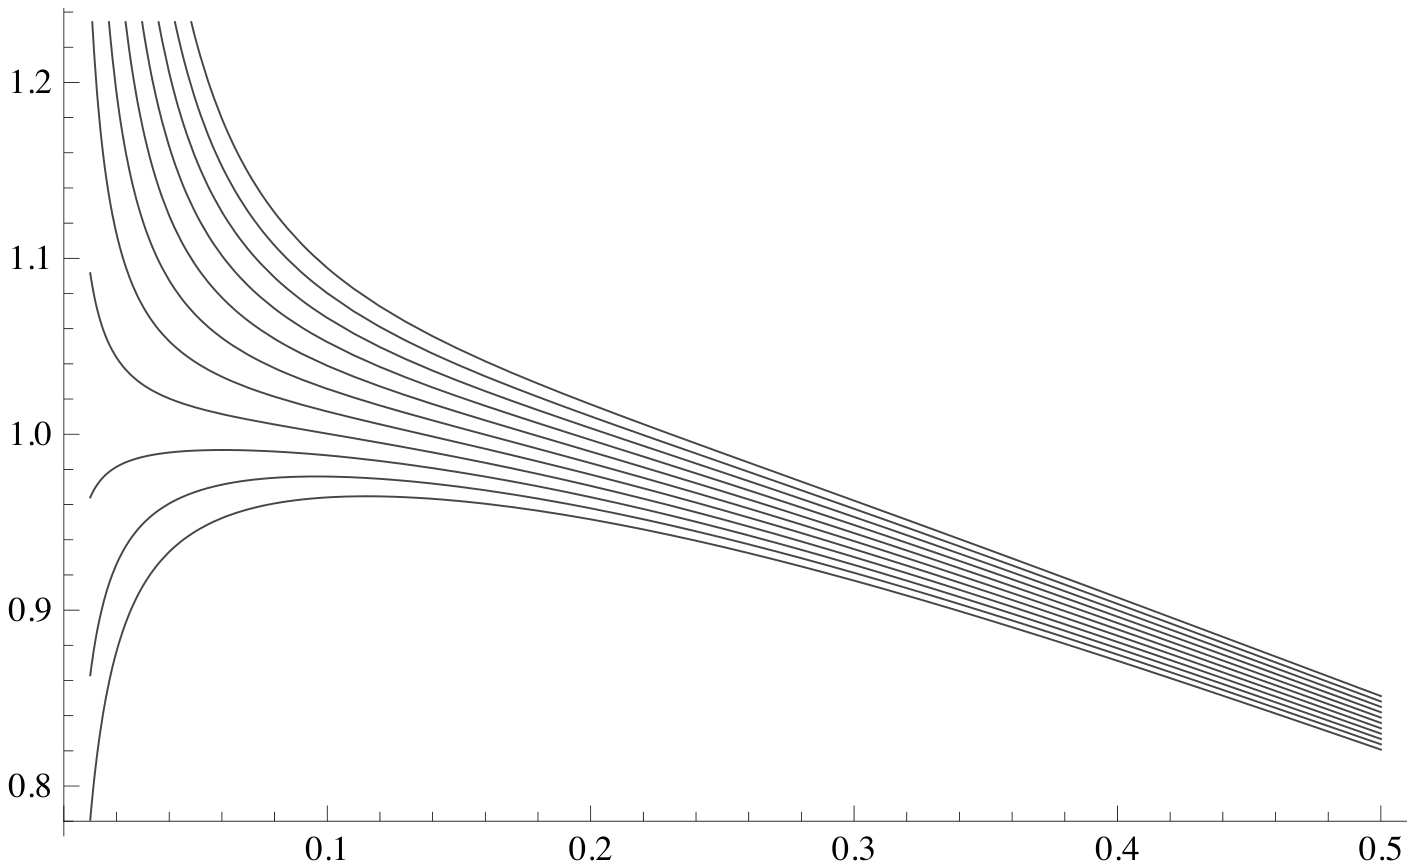
\includegraphics[width=3.5in]{figs/Fig29.png}
 \end{center}
\caption{\small  当 $\delta$ 跨过临界值变化时（取 $k=1$）的数值解。（原稿第 117 页）}
 \label{braidbo}
\end{figure}
